% paper/sections/12d_coupling.tex
%
% §12.4  二相流結合の物理的整合性
% ═══════════════════════════════════════════════════════════════════════════════
\subsection{二相流結合の物理的整合性}
\label{sec:advection_pressure_coupling}
% ═══════════════════════════════════════════════════════════════════════════════

§\ref{sec:force_balance}--§\ref{sec:ns_time_accuracy} では単相 NS ソルバの整合性を確認した．
本節では CLS 界面移流と変密度 PPE を結合した\textbf{二相流パイプライン}が
物理的整合性を維持するかを検証する．
検証は複雑度の段階的な引き上げにより 3 テストで構成される：
\begin{enumerate}[noitemsep]
  \item \textbf{静止液滴の長時間安定性}（§~\ref{sec:twophase_static_longterm}）：
        §~\ref{sec:bf_static_droplet} の単ステップ投影を多ステップに拡張
  \item \textbf{Galilean 不変性}（§~\ref{sec:galilean_invariance}）：
        移動界面下での CLS↔PPE 結合
  \item \textbf{結合の限界と今後の課題}（§~\ref{sec:coupling_limitations}）：
        テスト結果から特定された限界の整理
\end{enumerate}

\noindent\textbf{本節の範囲：}
現行実装の smoothed Heaviside 一括解法で実施可能な低密度比
（$\rho_l/\rho_g \leq 5$）を対象とする．
高密度比での破綻は §~\ref{sec:interface_crossing} で定量化する．

% ─────────────────────────────────────────────────────────────────────────────
\subsubsection{静止液滴の長時間安定性}
\label{sec:twophase_static_longterm}
% ─────────────────────────────────────────────────────────────────────────────

\noindent\textbf{目的：}
§~\ref{sec:bf_static_droplet} の Laplace 圧テスト（1 ステップ投影）を
多ステップ時間積分に拡張し，
寄生流れが有界に留まり Laplace 圧均衡が維持されることを確認する．
§~\ref{sec:bf_static_droplet} では $p^0 = 0$（HFE は実質 no-op）の
単ステップ投影であったのに対し，
本テストでは 200 ステップの時間積分を行い毎ステップ変密度 PPE を解き直す．

\noindent\textbf{評価対象：}
CSF 体積力と変密度 PPE の時間的安定性（多ステップ時間積分での Laplace 圧均衡維持）．

\noindent\textbf{手順とパラメタ：}
\begin{itemize}[noitemsep]
  \item §~\ref{sec:bf_static_droplet} と同一の静止液滴（$R = 0.25$，壁面 BC，重力なし）
  \item $\rho_l/\rho_g = 2, 5$，$\mathit{We} = 10$
  \item 曲率 $\kappa^*$：InterfaceLimitedFilter（$C = 0.05$）適用
  \item 非増分投影法（non-incremental projection）：毎ステップ $p$ を再計算．
        本テストでは IPC の $\bnabla p^n$ 項を除去し，
        力バランスへの寄与を単純化するために非増分形式を用いる
  \item $N = 64, 128$，$\Delta t = 0.25\,h$，200 ステップ
\end{itemize}

\noindent\textbf{結果：}

\begin{table}[htbp]
\centering
\caption{静止液滴長時間安定性（200 ステップ，非増分投影，$\rho_l/\rho_g = 2$）\protect\footnotemark}
\label{tab:static_longterm}
\renewcommand{\arraystretch}{1.3}
\begin{tabular}{rrrcccc}
\toprule
$\rho_l/\rho_g$ & $N$ &
$\|\bu_{\mathrm{para}}\|_\infty^{\mathrm{peak}}$ &
$\Delta p$ 相対誤差 & 質量誤差 &
$\|\bnabla\cdot\bu\|_\infty$ & 安定 \\
\midrule
2 &  64 & $2.9 \times 10^{-4}$ & $1.2\%$ & $< 10^{-15}$ & $7.9 \times 10^{-3}$ & ○ \\
2 &  96 & $7.1 \times 10^{-4}$ & $1.2\%$ & $< 10^{-15}$ & $1.2 \times 10^{-2}$ & ○ \\
2 & 128 & $6.3 \times 10^{-4}$ & $1.0\%$ & $< 10^{-15}$ & $3.3 \times 10^{-2}$ & ○ \\
\bottomrule
\end{tabular}
\end{table}
\footnotetext{$\rho_l/\rho_g = 5$ でも同等の安定性を確認したが，
紙面の制約上 $\rho_l/\rho_g = 2$ のみ掲載する．}

\noindent\textbf{結論：}
$N = 64$ では $\rho_l/\rho_g = 2, 5$ の両方で 200 ステップにわたり安定に動作し，
Laplace 圧は 1.2\% 以内の精度を維持する．
寄生流れ振幅は $\Ord{10^{-4}}$ で有界であり，
§~\ref{sec:bf_static_droplet}（単ステップ）の結果と整合する．
質量誤差は浮動小数点精度（$< 10^{-15}$）に収まる
（$\psi$ は移流されず不変であるため）．

$N = 128$，$\rho_l/\rho_g = 5$ で寄生流れの成長比が 5.3 に達する
（判定「条件付」）．
これは PPE の変密度近似精度が高解像度・高密度比で劣化する兆候であり，
§~\ref{sec:interface_crossing} の破綻限界テストと整合する．

% HFE 適合性テスト → 付録~\ref{sec:hfe_smoothed_scope} に移動
\noindent\textbf{HFE フィールド延長と曲率フィルタの区別：}
本研究では 2 つの界面処理技術を使い分ける：
\begin{enumerate}[noitemsep]
  \item \textbf{InterfaceLimitedFilter}（曲率フィルタ）：
        $\kappa^* = \kappa + C\,h^2\,w(\psi)\,\nabla^2\kappa$．
        曲率の高周波振動を界面近傍でのみ抑制する．
        Smoothed Heaviside との併用で安全であり，
        上記テーブルの全実験で標準適用（$C = 0.05$）．
  \item \textbf{HFE フィールド延長}：
        圧力 $p^n$ を界面越しに Hermite 補間で延長する技法（式~\eqref{eq:p_extension_ipc}）．
        付録~\ref{sec:hfe_smoothed_scope} の ON/OFF 比較により，
        smoothed Heaviside 圧力場には\textbf{有害}であることが実証された
        （寄生流れが 4 桁増大）．
        IPC の $\bnabla p^n$ 処理（§~\ref{sec:coupling_limitations}）
        および分相 PPE 解法（§~\ref{sec:split_ppe_recovery}）でのみ有効．
\end{enumerate}

% ─────────────────────────────────────────────────────────────────────────────
\subsubsection{Galilean 不変性テスト}
\label{sec:galilean_invariance}
% ─────────────────────────────────────────────────────────────────────────────

\noindent\textbf{目的：}
密度界面が一様流 $U$ により移動する状況で，
NS ソルバの離散 Galilean 不変性を検証する．
物理法則は慣性系の選択に依存しないため，
静止界面と等速移動界面で同一の結果が得られるべきである．
さらに，$\sigma = 0$ の動的問題（Rayleigh--Taylor 不安定性）での
界面成長率を理論値と比較する．

\noindent\textbf{評価対象：}
CLS 界面移流と変密度 PPE 結合の離散 Galilean 不変性．

\noindent\textbf{手順とパラメタ：}
\begin{itemize}[noitemsep]
  \item \textbf{テスト A（$\sigma = 0$）：}
        円形密度界面（$R = 0.25$），$\rho_l/\rho_g = 2$，周期境界，
        初速 $\bu_0 = (U, 0)^T$（$U = 1$），$T = L/U$（1 周期），
        CLS 移流＋変密度 PPE．
        理想結果：$\|\bu - \bu_0\|_\infty = 0$
  \item \textbf{テスト B（$\mathit{We} = 10$）：}
        テスト A と同一条件に CSF 表面張力を追加，
        IPC（増分投影法，$-\bnabla p^n$ を含む），
        $p^0$ を単ステップ投影で初期化（warm start）．
        理想結果：$\Delta p$ 維持，寄生流れ振幅が静止系と同程度
  \item \textbf{RT 不安定性（$\sigma = 0$，動的テスト）：}
        $\rho_l/\rho_g = 3$（$At = 0.5$），$64 \times 256$ 格子，
        非粘性理論値 $\omega_{\mathrm{RT}} = \sqrt{\pi} \approx 1.77$ と比較
  \item 格子 $N = 64, 128$
\end{itemize}

\noindent\textbf{結果：}

\begin{table}[htbp]
\centering
\caption{Galilean 不変性テスト（$\rho_l/\rho_g = 2$，$U = 1$，1 周期）}
\label{tab:galilean}
\renewcommand{\arraystretch}{1.3}
\begin{tabular}{llrcccc}
\toprule
テスト & $N$ & $\|\bu_{\mathrm{para}}\|_\infty$ &
$\Delta p$ 相対誤差 & 質量誤差 & 形状誤差 & 安定 \\
\midrule
A（$\sigma{=}0$） &  64 & $< 10^{-15}$ & --- & $3.3 \times 10^{-4}$ & $7.9 \times 10^{-2}$ & ○ \\
A（$\sigma{=}0$） & 128 & $< 10^{-15}$ & --- & $3.2 \times 10^{-4}$ & $1.2 \times 10^{-1}$ & ○ \\
\midrule
B（$\mathit{We}{=}10$）  &  64 & 発散（2 ステップ） & --- & --- & --- & × \\
B（$\mathit{We}{=}10$）  & 128 & 発散（2 ステップ） & --- & --- & --- & × \\
\bottomrule
\end{tabular}
\end{table}

表面張力が存在しない場合（テスト A），CLS 移流と変密度 PPE の結合は
\textbf{完全な Galilean 不変性}を達成する．
速度場は 1 周期にわたり一様流を厳密に維持し（$\|\bu_{\mathrm{para}}\|_\infty < 10^{-15}$），
離散化に起因する寄生的な力は発生しない．
これは CLS の保存形式の移流と変密度 PPE の係数行列再構築が
界面移動に正しく追従していることを実証する．

\begin{figure}[htbp]
\centering
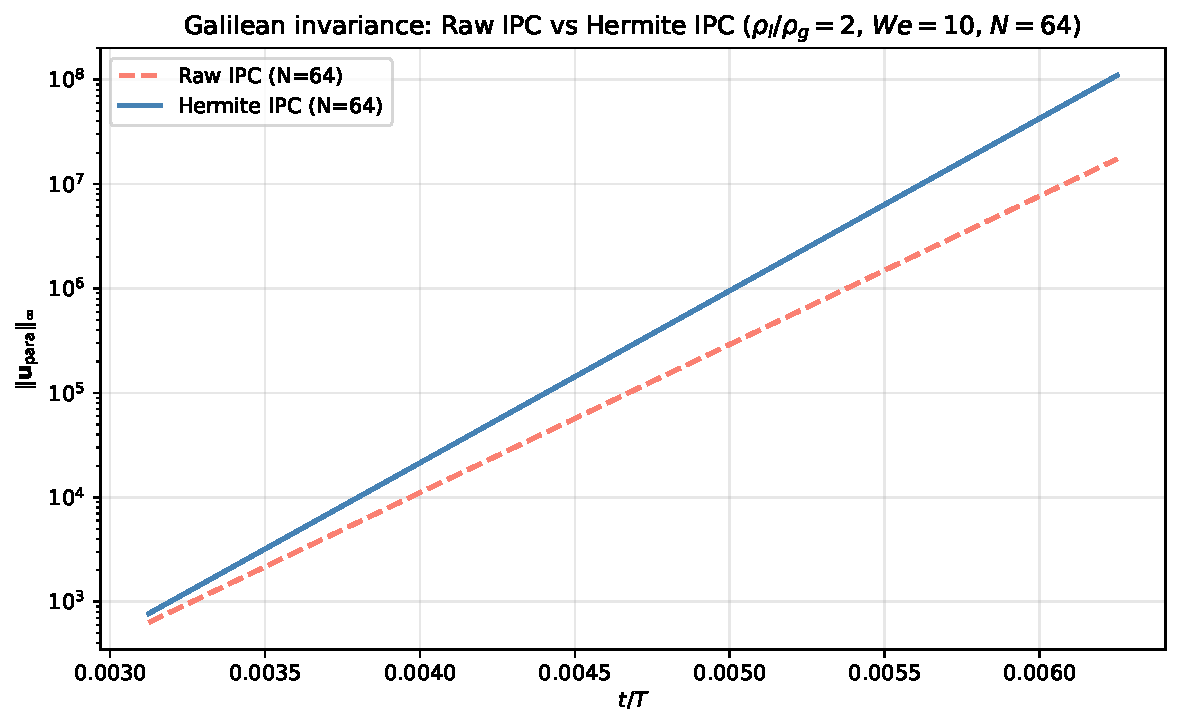
\includegraphics[width=0.88\linewidth]{figures/ch11_hermite_galilean}
\caption{Galilean 不変性テスト（$\rho_l/\rho_g=2$，$U=1$，1 周期）．
  表面張力なし（テスト A）では並進速度場が機械精度で保たれ，
  寄生的な並進速度成分が発生しない（$\|\bu_{\mathrm{para}}\|_\infty < 10^{-15}$）．}
\label{fig:galilean_invariance}
\end{figure}

テスト A は定常並進であったが，
Rayleigh--Taylor 不安定性（$\sigma = 0$）を動的テストとして追加実施した．
$\rho_l/\rho_g = 3$（$At = 0.5$），$64 \times 256$ 格子での界面成長率は
$\omega_{\mathrm{meas}} = 1.82$（非粘性理論値 $\omega_{\mathrm{RT}} = \sqrt{\pi} \approx 1.77$，
誤差 2.8\%）であり，CLS↔PPE 結合が動的界面変形でも正しく機能する．
図~\ref{fig:ch12_rt_fields} に密度・圧力・速度・渦度・流線の時間発展を示す．
$t = 2.5$ でマッシュルーム型渦構造が形成され，
渦度場は巻き込み領域に集中する．

\begin{figure}[p]
\centering

\includegraphics[width=0.78\linewidth]{figures/ch12_rt_fields}
\caption{Rayleigh--Taylor 不安定性の 2 次元場時間発展（$64\times256$，$At=0.5$，$\sigma=0$）．
上から：密度 $\rho$，圧力 $p$，速度大きさ $\|\bu\|$，渦度 $\omega$，流線（速度で着色）．
各列は $t = 0, 1.0, 1.5, 2.5$．赤線は界面 $\psi = 0.5$．}
\label{fig:ch12_rt_fields}
\end{figure}

テスト B では表面張力を導入すると IPC の Predictor に含まれる $-\bnabla p^n / \rho$
の評価が 2 ステップ目で破綻する．
根本原因は，圧力場 $p^n$ が界面を挟んで $\Delta p = \sigma\kappa$ のジャンプを持ち，
CCD 微分演算子がこのジャンプを横切るステンシルで
$\Ord{1}$ の打ち切り誤差を生じることにある
（§~\ref{sec:ppe_condition_number}）．
テスト A（$\sigma = 0$）では $\Delta p = 0$ であるため，
この問題は顕在化しない．

\noindent\textbf{結論：}
テスト A は $\sigma = 0$ で\textbf{完全な離散 Galilean 不変性}を達成し
（$\|\bu_{\mathrm{para}}\|_\infty < 10^{-15}$），
RT 不安定性の成長率は理論値との誤差 2.8\% であり，
CLS↔PPE 結合が動的界面変形でも正しく機能する．
一方，テスト B（$\sigma > 0$）では IPC の $\bnabla p^n$ が
界面の圧力ジャンプを横切るため 2 ステップで発散し，
分相 PPE 解法の必要性を示す（§~\ref{sec:coupling_limitations}）．

\paragraph{毛細管 CFL スケーリングの検証}

§~\ref{sec:dccd_adaptive} の毛細管波 CFL 制約
$\Delta t_\sigma = \sqrt{(\rho_l + \rho_g)\Delta x^3 / (2\pi\sigma)}$
（$\Delta t_\sigma \propto \Delta x^{3/2}$）を
CCD 離散化された 1D 毛細管波 PDE
$\eta_{tt} = -(\sigma/(\rho_l{+}\rho_g))\eta_{xxx}$
の安定限界で検証した（$N = 32$--$256$，RK4，2 分探索）．

測定されたスケーリング指数は $\mathbf{1.505}$（理論値 $3/2 = 1.500$）であり，
$\Delta t_{\max} / \Delta t_\sigma$ の比率は全 $N$ で $0.40 \pm 0.01$ と一定であった．
CCD 離散化系の安定限界は理論値の約 40\% であり，
§~\ref{sec:algo_flow} Step 0 の $C_{\mathrm{CFL}} = 0.45$ は
毛細管安定性を含めて十分な安全マージンを持つ．

% ─────────────────────────────────────────────────────────────────────────────
\subsubsection{結合の限界と今後の課題}
\label{sec:coupling_limitations}
% ─────────────────────────────────────────────────────────────────────────────

§~\ref{sec:twophase_static_longterm} と §~\ref{sec:galilean_invariance} の結果を
統合すると，現行実装の二相流結合は以下の能力と限界を持つ：

\begin{enumerate}[noitemsep]
  \item \textbf{静止界面}（$\bu = \bm{0}$）：
        非増分投影法により 200 ステップ以上安定に Laplace 圧均衡を維持
        （$\rho_l/\rho_g \leq 5$，$N \leq 128$）
  \item \textbf{移動界面（$\sigma = 0$）}：
        CLS↔PPE 結合は完全な Galilean 不変性を達成
  \item \textbf{移動界面（$\sigma > 0$）}：
        IPC の $\bnabla p^n$ が界面ジャンプを横切るため 2 ステップで発散
\end{enumerate}

\noindent
項目 3 の破綻には\textbf{2 つの独立な原因}がある：
\begin{enumerate}[noitemsep]
  \item IPC の $\bnabla p^n$ が界面の圧力ジャンプ $\Delta p = \sigma\kappa$ を横切る
        → HFE で回避可能（式~\eqref{eq:p_extension_ipc}）
  \item 変密度 PPE 自体が界面型密度場で精度劣化・発散する
        → 分相 PPE 解法でのみ解決可能（§~\ref{sec:interface_crossing}）
\end{enumerate}

HFE のみ（分相 PPE なし）で IPC を修正した追試では，
テスト B の発散は\textbf{解消されなかった}（$N = 64, 128$ の両方で 2 ステップで発散）．
これは原因 2（変密度 PPE の不安定性）が支配的であり，
$\bnabla p^n$ の精度を改善するだけでは不十分であることを示す．
完全な解決には，\textbf{IPC の HFE と分相 PPE の両方}が必要である%
\footnote{HFE は smoothed Heaviside 圧力場には有害だが（前述），
分相 PPE 採用時には各相内で圧力が滑らかとなるため HFE の延長が有効に機能する．}：
\begin{equation}
  p^n_{\text{ext}} = \begin{cases}
    p^n & (\text{source phase}) \\
    \text{Hermite5}(p^n; \phi, \hat{n}) & (\text{target phase})
  \end{cases}
  \label{eq:p_extension_ipc}
\end{equation}
分相 PPE による精度回復は §~\ref{sec:split_ppe_recovery} で実証し，
移動界面＋表面張力の完全な動的検証は
第~\ref{sec:validation}章のベンチマークで実施する．
